\documentclass{acm_proc_article-sp}
\pagenumbering{arabic}

\usepackage{epstopdf}
\usepackage{etoolbox}
\usepackage{listings}

\usepackage{multirow}
\usepackage{caption}
\usepackage{epstopdf}
\usepackage{float}
\usepackage[hyphens]{url}
\usepackage{etoolbox}
\usepackage{color}
\usepackage{listings}
\usepackage{lscape}
\usepackage{enumitem}
\lstset{ %
language={[x86masm]Assembler},                % choose the language of the code
basicstyle=\footnotesize,       % the size of the fonts that are used for the code
numbers=left,                   % where to put the line-numbers
numberstyle=\footnotesize,      % the size of the fonts that are used for the line-numbers
stepnumber=1,                   % the step between two line-numbers. If it is 1 each line will be numbered
numbersep=5pt,                  % how far the line-n/umbers are from the code
backgroundcolor=\color{white},  % choose the background color. You must add \usepackage{color}
showspaces=false,               % show spaces adding particular underscores
showstringspaces=false,         % underline spaces within strings
showtabs=false,                 % show tabs within strings adding particular underscores
frame=single,           % adds a frame around the code
tabsize=2,          % sets default tabsize to 2 spaces
captionpos=b,           % sets the caption-position to bottom
breaklines=true,        % sets automatic line breaking
breakatwhitespace=false,    % sets if automatic breaks should only happen at whitespace
escapeinside={\%*}{*)}          % if you want to add a comment within your code
}

\makeatletter
\patchcmd{\maketitle}{\@copyrightspace}{}{}{}
\makeatother


\begin{document}

% Marmar got really tired of typing privacy policy/policies, so \newcommand please
\newcommand{\pp}{privacy policy}
\newcommand{\pps}{privacy policies}

\title{COS 597D Project - Mobile vs Traditional Web Tracking\\(FourthPartyMobile)}
%
% You need the command \numberofauthors to handle the 'placement
% and alignment' of the authors beneath the title.
%
% For aesthetic reasons, we recommend 'three authors at a time'
% i.e. three 'name/affiliation blocks' be placed beneath the title.
%
% NOTE: You are NOT restricted in how many 'rows' of
% "name/affiliations" may appear. We just ask that you restrict
% the number of 'columns' to three.
%
% Because of the available 'opening page real-estate'
% we ask you to refrain from putting more than six authors
% (two rows with three columns) beneath the article title.
% More than six makes the first-page appear very cluttered indeed.
%
% Use the \alignauthor commands to handle the names
% and affiliations for an 'aesthetic maximum' of six authors.
% Add names, affiliations, addresses for
% the seventh etc. author(s) as the argument for the
% \additionalauthors command.
% These 'additional authors' will be output/set for you
% without further effort on your part as the last section in
% the body of your article BEFORE References or any Appendices.

\numberofauthors{1} %  in this sample file, there are a *total*
% of EIGHT authors. SIX appear on the 'first-page' (for formatting
% reasons) and the remaining two appear in the \additionalauthors section.
%
\author{
% You can go ahead and credit any number of authors here,
% e.g. one 'row of three' or two rows (consisting of one row of three
% and a second row of one, two or three).
%
% The command \alignauthor (no curly braces needed) should
% precede each author name, affiliation/snail-mail address and
% e-mail address. Additionally, tag each line of
% affiliation/address with \affaddr, and tag the
% e-mail address with \email.
%
% 1st. author
\alignauthor
Marcela Melara, Christian Eubank and Diego Perez Botero \\ 
       \email{\{melara, cge, diegop\}@princeton.edu}
}

\maketitle

\begin{abstract}
INSERT ABSTRACT HERE??
\end{abstract}

\category{H.3.5}{Information Systems}{Information Storage and Retrieval}[Web-based services]
\category{K.4.1}{Computing Milieux}{Computers and Society}[Privacy]

\terms{Documentation, Measurement, Security}

\keywords{FourthParty, Web crawling, cookies, privacy policy, ...}

\section{Introduction}
We wish to automate the detection of third-party tracking mechanisms while browsing the web on a mobile device. To this end, we will adopt the FourthParty\footnote{http://www.fourthparty.info} project's approach and instrument a popular open-source mobile browser (i.e. Firefox) to be used as an enhanced web crawler. This enables us to log realistic end-user interactions (e.g. execution of embedded scripts) as opposed to just downloading each web page's static content, which is what traditional web crawlers do.

The mobile web crawler is the tool that we will use to collect valuable information in order to conduct our comparison between the Mobile and Traditional third-party tracking ecosystems and their practices.


\section{Background and Motivation}

\section{Related Work}
MARCELA

\section{Implementation}
This section explains the design decisions and the software development process that the FourthPartyMobile project entailed.

\subsection{Challenges}
Mobile application development poses a variety of challenges that will need to be addressed for a mobile web crawler to be materialized:

\begin{itemize}
\item Mobile devices have limited amounts of RAM, so applications should not rely on large data structures stored in main memory.

\item Security permissions in mobile devices are strict, which means that writing data into persistent memory is not always an option.

\item Processing power in mobile devices is limited, so computationally intensive procedures, such as parsing a web page, should be delegated to an external entity.

\item Mobile network bandwidth is a limited resource, so large data transfers should be avoided.

\item Battery life must be preserved as much as possible by a mobile application if it is being aimed towards the general public.
\end{itemize}


\subsection{Mobile Web Crawler's Architecture}

FourthPartyMobile's architecture (see Figure \ref{fig:component_diagram}) delegates most of the computation and storage to a supporting server, limiting the mobile device's responsibilities to fetching one website at a time and generating a log of its latest interactions (e.g. cookies, JavaScript, embedded HTTP objects). The crawling plugin running on the mobile device sends the interaction log corresponding to the website being visited in the form of SQL statements to the crawling backend running on a server. This way, the amount of state kept in the mobile device's main memory is minimal and the crawl database, which can be several Megabytes in size, is generated by the supporting server's side. 

\begin{figure}[h] 
\centering 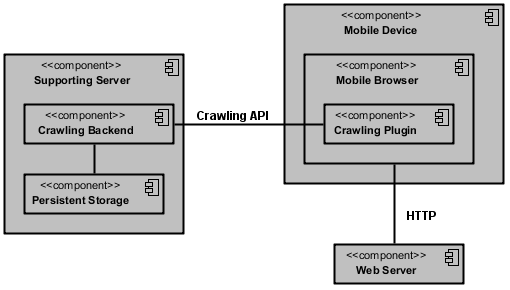
\includegraphics[scale=0.65]{diagrams/component_diagram.png}
\caption{Prototype's Runtime Interactions.}
\label{fig:component_diagram}
\end{figure}



\subsection{Prototype}
We took advantage of the fact that the FourthParty\footnote{http://www.fourthparty.info} project is open-source. After analyzing its codebase, we ported its core functionality over to support Android-based mobile devices, such as smartphones and tablets. FourthPartyMobile is implemented in Java and JavaScript, leveraging both the Android SDK and the Mozilla Add-On SDK. Persistent storage is fully compliant with FourthParty's SQLite database schema. Thus, we provide a standardized representation for traditional and mobile crawls, which facilitates data analysis. Our Crawling Backend is written in java with a SQLite JDBC library that supports Mac OS, Linux and Windows, so it should be fully multi-platform. It also supports concurrency, so multiple crawls can be recorded simultaneously. 

The FourthPartyMobile code was the end result of four development phases:

\begin{enumerate}
\item \textbf{Code Refactoring}: the original FourthParty source code had to be refactored to comply with Mozilla Add-On SDK 1.5+ and Javascript 1.8+. This was done by repeatedly pushing the code to an Android device and analyzing its Exception traces.

\item \textbf{Architectural Changes}: the refactored source code was changed to remove its dependencies on local secondary storage and all persistence operations were redirected to a TCP connection.

\item \textbf{Support Infrastructure}: the support server and other necessary tools (e.g. crawl scripts generator) were developed.

\item \textbf{Testing}: FourthPartyMobile was deployed in different devices and various test crawls were conducted to identify and eliminate all remaining bugs.

\end{enumerate}

\section{Methodology}
This section details the steps we took to ensure that our results are highly reproducible. It also describes our test bed and the reasoning behind it.


\begin{figure*}[ht] 
\centering 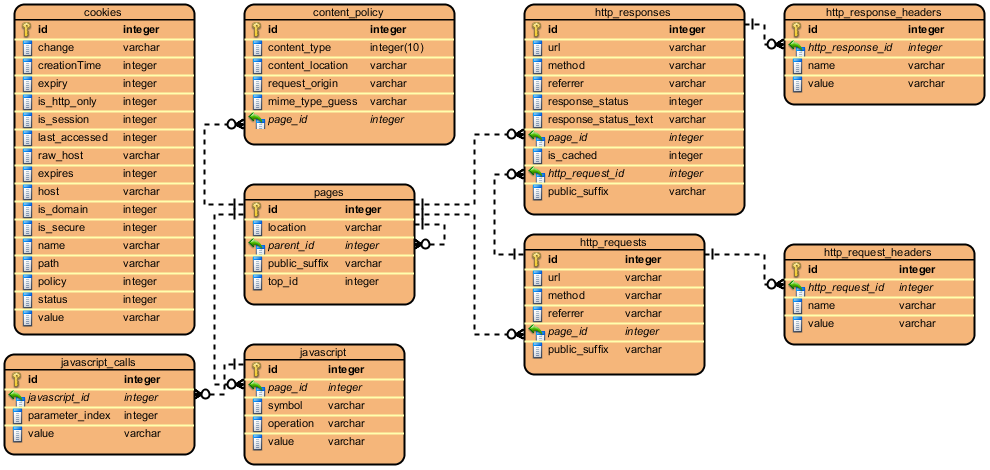
\includegraphics[scale=0.70]{diagrams/db_diagram.png}
\captionof{figure}{FourthParty SQLite database schema}
\label{fig:db_schema}
\end{figure*}

\subsection{Automated Crawls}

We tried automating crawls on Firefox Mobile with MozMill\footnote{https://developer.mozilla.org/en-US/docs/Mozmill}, Selenium\footnote{http://seleniumhq.org/}, Scriptish\footnote{http://scriptish.org/} and Robocop\footnote{https://quality.mozilla.org/browser-technologies/mobile-firefox/robocop/} without any success. The few frameworks that are compatible with Android do not support Firefox Mobile (fennec) -- they only interact with the lackluster Android Web Browser. To the best of our knowledge (i.e. hours worth of Google searches), it seems that there are no testing frameworks out there that can automate Firefox Mobile crawls. Even the browser plugins that do this on the desktop version (e.g. Flem\footnote{https://addons.mozilla.org/en-US/firefox/addon/flem/}) have not been ported to the Mozilla Mobile SDK. Bare in mind that Mozilla Mobile SDK was released on February 21 of 2012 \cite{announcing_sdk}, so it needs more time to mature.

Our solution was to use JavaScript code on one site to trigger the crawl on a separate tab. We tested this method on all platforms (i.e. desktop, tablet, smartphone) with positive results. Thus, we automated the generation of the HTML website containing the JavaScript code to facilitate the creation of these scripts for arbitrary URL lists. A timeout of 30 seconds was used for every one of our crawls, meaning that a new URL was visited every 30 seconds.

\subsection{URL Datasets}

We crawled two URL datasets parsed from \emph{Alexa - Top Sites in United States} on January 7, 2013: (1) Top 100 and (2) Top 500. Our decision to focus on the Top US Sites instead of the Top Global Sites came after a series of crashes were caused by websites containing non-western character sets.

\subsection{Devices}

All crawls were conducted between January 7, 2013 and January 10, 2013. Six different devices were used to go through the two URL datasets, for a total of 12 result sets. We used one PC, one smartphone and two tablets, as well as an emulated smartphone and an emulated tablet:

\begin{itemize}\itemsep0em 
\item Desktop (Ubuntu 12.04, Firefox 11.0)

\item Asus Transformer Pad TF300T (10.1-inch Tablet)

\item Samsung Galaxy Tab 2 (7.0-inch Tablet)

\item Emulated Nexus 7 (7.0-inch Tablet)

\item HTC Evo 4G (4.8-inch Smartphone)

\item Emulated Nexus S (4.0-inch Smartphone)
\end{itemize}

The two emulated devices were created with the Android Virtual Device (AVD) tool that comes with the Android SDK. We tweaked the emulator's settings in order to create an Android smartphone and tablet that were as close as possible to their physical equivalents. Four non-generic system images are packed with the Android 4.2 API SDK tools: Nexus 7 (tablet), Galaxy Nexus (phone), Nexus S (phone) and Nexus One (phone).  Therefore, we believe that they provide the most accurate runtime environments when trying to impersonate physical devices. Out of all the phone images, the Nexus S shared the most similarities with the HTC Evo 4G in terms of their technical specifications, so it was deemed more accurate than the other two options.

\subsection{FourthParty SQLite Database Schema}
Figure \ref{fig:db_schema} shows the database schema generated on every crawl. The \emph{cookies} table is self-contained and describes all the cookie-related creation, modification and deletion events, along with the host responsible for each event, the value written to the cookie, and other interesting metadata. JavaScript execution details are divided into the \emph{javascript} and \emph{javascript\_calls} tables, where the former lists the functions triggered by the scripts and the latter stores the arguments given to those functions. On the HTTP side, the \emph{http\_requests} table lists each HTTP Request's basic information and is complemented by the \emph{http\_request\_headers} table, which contains all of the corresponding HTTP headers and their values. A similar arrangement exists for HTTP Responses. Lastly, the \emph{pages} and \emph{content\_policy} tables are concerned with the location of the content being sent to the user's browser and the pages responsible for it.

Unfortunately, the mobile-enabled Mozilla Add-On SDK currently lacks support for the types of hooks required to properly intercept JavaScript calls and content\_policy invocations. For this reason, the SQLite tables specifically allocated for JavaScript traces and content\_policy logs are never populated during our crawls. However, HTTP responses state their content type in the headers and all JavaScript code is transferred to the browser through HTTP responses. Thus, a simple query like the one shown in Listing 1 reveals the HTTP responses associated with that sort of code. By leveraging the power of SQL queries, we were able to carry out very detailed analyses related to JavaScript code in spite of the absence of the \emph{javascript} and \emph{javascript\_calls} tables (refer to Section 6).

\noindent\begin{minipage}{1.0\linewidth}\centering
\begin{lstlisting}[caption=Example JavaScript analysis based on HTTP Responses]
SELECT *
FROM http_response_headers
WHERE UPPER(name)='CONTENT-TYPE' AND value LIKE '%javascript%'
\end{lstlisting}
\end{minipage}

\section{Data Analysis}

\subsection{Main Players}

In determining the sites with the most prevalent tracking habits, we first considered those sites who added the most cookies during the crawl. Specifically, we considered those sites who were in (or tied with) the top 25 for each device in terms of the number of cookies added in the 500-site crawl. Notably, third-party advertising and analytics sites comprised a sizable minority of the top 25 cookie-adders, forming 34.6\% of the top 25 for desktops, 39.3\% for tablets and 30.8\% for phones. The majority of first-party cookie adders were online retailers and news sites.

As recorded in Table~\ref{tab:major_cookies}, roughly one third of the top cookie-adders were ranked highly across all three types of devices. Differences in the top cookie-adders across the three devices were partially a relic of third-party websites that added cookies heavily on one platform, but not the others. Interestingly, tablets appeared to lie in between phones and computers in terms of top advertising/analytics cookie-adders. Specifically, among others, the tablet shared \texttt{2o7.net} and \texttt{collective-media.net} with phones and \texttt{dotomi.com} and \texttt{rfihub.com} with desktops. In contrast, phones and desktops did not share a top analytics/advertiser in their top 25 that did not also appear in the top 25 for tablets.


\begin{table}[htbp]
  \centering
  \caption{Cookie-adding websites in top 25 for all devices}
    \begin{tabular}{|c|c|c|c|}
    \hline
     \multicolumn{1}{|l|}{\textbf{Website}} & \textbf{Description}    \\ \hline
    \multicolumn{1}{|l|}{\texttt{cafepress.com}} & Online retailer   \\
    \multicolumn{1}{|l|}{\texttt{go.com}} & Disney-owned web portal  \\
    \multicolumn{1}{|l|}{\texttt{homedepot.com}} & Online retailer    \\
    \multicolumn{1}{|l|}{\texttt{hootsuite.com}} & Social media management site   \\
    \multicolumn{1}{|l|}{\texttt{pubmatic.com}} & Online advertising company   \\
    \multicolumn{1}{|l|}{\texttt{revsci.net}} & Shell for advertiser Audience Science    \\
    \multicolumn{1}{|l|}{\texttt{rubiconproject.com}} & Online advertising company   \\
    \multicolumn{1}{|l|}{\texttt{verizon.com}} & Telecommunications/ online retailer   \\
    \multicolumn{1}{|l|}{\texttt{webs.com}} & Web hosting services  \\ \hline
    \end{tabular}%
  \label{tab:major_cookies}%
\end{table}%

The next metric for tracking that we considered was the number of JavaScript calls made by one site that refer to another site. In most cases, these calls were to third-party advertisers and analytic organizations. These organizations were largely completely separate third-parties, but in cases such as \texttt{washingtonpost.com} and \texttt{wapolabs.com}, the first and  ``third" parties were actually part of the same umbrella organization. 

Websites in the top 25 for containing JavaScript calls by other websites for all three types of devices are contained Table~\ref{tab:major_js}. Observe that these sites are predominately news and retailing sites, a trend that held for the websites not included in the table. However, beyond these 6 sites, the three devices only shared a small handful of sites in their JavaScript top 25, unlike in the case of cookie-adders.

Overall, based on our cookie and JavaScript analysis, news media and online retailers appear to be the most pervasive first-party trackers while third-party advertisers and analytics groups have a notable presence on all three types of devices.

\begin{table}[htbp]
  \centering
  \caption{Websites in Top 25 for all devices for containing JS referring to other sites}
    \begin{tabular}{|c|c|c|c|}
    \hline
     \multicolumn{1}{|l|}{\textbf{Referrer}} & \textbf{Description}    \\ \hline
     \multicolumn{1}{|l|}{\texttt{cbslocal.com}} & Online news site   \\
    \multicolumn{1}{|l|}{\texttt{drudgereport.com}} & Online news site   \\
     \multicolumn{1}{|l|}{\texttt{mypoints.com}} & Online reward-points retailer   \\
      \multicolumn{1}{|l|}{\texttt{theblaze.com}} & Online news site   \\
       \multicolumn{1}{|l|}{\texttt{time.com}} & Online news site   \\
        \multicolumn{1}{|l|}{\texttt{verizonwireless.com}} & Telecommunications/ online retailer   \\ \hline
    \end{tabular}%
  \label{tab:major_js}%
\end{table}%

\subsection{Desktop vs Mobile Tracking}

As when examining the major players in tracking, we compared desktop and mobile devices with respect to an investigation of the cookies and JavaScript calls observed during the crawls. Tables~\ref{tab:dm_cookie_counts_100} and~\ref{tab:dm_cookie_counts_500} contain the raw number of cookie-related calls for the devices. Unsurprisingly, as the devices became smaller and more mobile, the number of cookies added during the crawls decreased, likely due to space constraints. However, when considering the proportion of cookies left on a device after the crawls, cookies appear to be stickier in the short term on the more mobile devices. This result is likely due to the fact that, since trackers can add a smaller number of cookies on a mobile device, they try to keep the few cookies they place on the device as long as possible.

Another basic way to categorize cookies' longevities is by their expiration time: some are evicted from the browser's memory after a finite amount of time, while others are meant to stay in the browser's memory permanently. Permanent cookies are set by Mozilla Firefox to expire after exactly 9.223372036854776 * $10^{18}$ milliseconds; temporary cookies have eviction times that are more manageable (e.g. 11 days). The results of examining the expiration dates are contained in Table~\ref{tab:dm_cookie_longeivity}. Note that, as with short-term cookie stickiness, the proportion of permanent cookies increases as devices become more mobile.


\begin{table}[htbp]
  \centering
  \caption{Desktop v. mobile cookie action counts with Top 100 dataset}
    \begin{tabular}{|c|c|c|c|c|}
    \hline
    \multicolumn{1}{|c|}{\multirow{2}[4]{*}{\textbf{Device}}} & \multicolumn{4}{|c|}{\textbf{Cookies - Top 100 Dataset}} \\ \cline{2-5}
    \multicolumn{1}{|c|}{} & \multicolumn{1}{|c|}{\textbf{Added}} & \multicolumn{1}{|c|}{\textbf{Changed}} & \multicolumn{1}{|c|}{\textbf{Deleted}} & \multicolumn{1}{|c|}{\textbf{\% Left}}\\ \hline
    \multicolumn{1}{|l|}{\textbf{Desktop}} & 1732   & 2605  & 148 & 91.45\% \\
    \multicolumn{1}{|l|}{\textbf{Tablet (avg).}} & 1233.5  & 1922.5  & 107 & 91.32\%\\
    \multicolumn{1}{|l|}{\textbf{Phone}} & 936   & 1214  & 18 & 98.08\% \\ \hline
    \end{tabular}%
  \label{tab:dm_cookie_counts_100}%
\end{table}%

\begin{table}[htbp]
  \centering
  \caption{Desktop v. mobile cookie action counts with Top 500 dataset}
    \begin{tabular}{|c|c|c|c|c|}
    \hline
    \multicolumn{1}{|c|}{\multirow{2}[4]{*}{\textbf{Device}}} & \multicolumn{4}{|c|}{\textbf{Cookies - Top 500 Dataset}} \\ \cline{2-5}
    \multicolumn{1}{|c|}{} & \multicolumn{1}{|c|}{\textbf{Added}} & \multicolumn{1}{|c|}{\textbf{Changed}} & \multicolumn{1}{|c|}{\textbf{Deleted}} & \multicolumn{1}{|c|}{\textbf{\% Left}}\\ \hline
\multicolumn{1}{|l|}{\textbf{Desktop}} & 7355  & 13174  & 640 & 91.30\%\\
    \multicolumn{1}{|l|}{\textbf{Tablet (avg.)}} & 5396.5  & 6845.5  & 262 & 95.15\%\\
    \multicolumn{1}{|l|}{\textbf{Phone}} & 4387  & 4545  & 101 & 97.70\%\\ \hline
    \end{tabular}%
  \label{tab:dm_cookie_counts_500}%
\end{table}%

\begin{table}[htbp]
  \centering
  \caption{Desktop v. mobile cookie longevity with Top 500 dataset}
    \begin{tabular}{|c|c|c|c|c|}
    \hline
    \multicolumn{1}{|c|}{\multirow{2}[4]{*}{\textbf{Device}}} & \multicolumn{4}{|c|}{\textbf{Cookies - Top 500 Dataset}} \\ \cline{2-5}
    \multicolumn{1}{|c|}{} & \textbf{Perm.} & \textbf{Temp.} & \textbf{\% Perm.} & \textbf{Total} \\ \hline
    \multicolumn{1}{|l|}{\textbf{Desktop}} & 4962  & 16527  & 23.09\% & 21489 \\
    \multicolumn{1}{|l|}{\textbf{Tablet (avg).}} & 3571.5  & 8932.5  & 28.56\% & 12504 \\
    \multicolumn{1}{|l|}{\textbf{Phone}}  & 2805  & 6228  & 31.05\% & 9033 \\  \hline
    \end{tabular}%
  \label{tab:dm_cookie_longeivity}%
\end{table}%

Next we turn to the number of JavaScript calls, including the third-party JavaScript calls. We define third-party JavaScript calls as in the previous section. Observe, in Tables~\ref{tab:dm_javascript_100} and~\ref{tab:dm_javascript_500} that the raw number of JavaScript calls as well as the proportion of calls by third-party entities fall from desktop to tablet to mobile phone. This suggests, from a tracking point of view, that JavaScript is increasingly used for purposes more in accordance with site mechanics (e.g. rendering) as opposed to tracking as devices move in the mobile direction. This could be a relic of the fact that, since these mobile devices lack the same computing power as desktops, adding extra JavaScript for purposes other than running the first-party content would slow browsing down to an unacceptable degree. Hence, one could hypothesize that, in general, trackers will use cookies (which do not require significant computational power) more frequently when compared to JavaScript on mobile devices.


\begin{table}[htbp]
  \centering
  \caption{JavaScript call counts with Top 100 dataset}
    \begin{tabular}{|c|c|c|c|}
    \hline
    \multicolumn{1}{|c|}{\multirow{2}[4]{*}{\textbf{Device}}} & \multicolumn{3}{|c|}{\textbf{JavaScript Calls - Top 100 Dataset}} \\ \cline{2-4}
    \multicolumn{1}{|c|}{} & \multicolumn{1}{|c|}{\textbf{Total}} & \multicolumn{1}{|c|}{\textbf{3rd Party}} & \multicolumn{1}{|c|}{\textbf{\% 3rd Party}}  \\ \hline
    \multicolumn{1}{|l|}{\textbf{Desktop}} & 1763   & 1238  & 70.22\% \\
    \multicolumn{1}{|l|}{\textbf{Tablet (avg.)}} & 1244.5   & 864 & 69.43\%  \\
    \multicolumn{1}{|l|}{\textbf{Phone}} & 798  & 454  & 56.89\% \\ \hline
    \end{tabular}%
  \label{tab:dm_javascript_100}%
\end{table}%

\begin{table}[htbp]
  \centering
  \caption{JavaScript call counts with Top 500 dataset}
    \begin{tabular}{|c|c|c|c|}
    \hline
    \multicolumn{1}{|c|}{\multirow{2}[4]{*}{\textbf{Device}}} & \multicolumn{3}{|c|}{\textbf{JavaScript Calls - Top 500 Dataset}} \\ \cline{2-4}
    \multicolumn{1}{|c|}{} & \multicolumn{1}{|c|}{\textbf{Total}} & \multicolumn{1}{|c|}{\textbf{3rd Party}} & \multicolumn{1}{|c|}{\textbf{\% 3rd Party}} \\ \hline
    \multicolumn{1}{|l|}{\textbf{Desktop}} & 10912   & 7310  & 66.99\% \\
    \multicolumn{1}{|l|}{\textbf{Tablet (avg.)}} & 6165   & 3848  & 62.42\% \\
    \multicolumn{1}{|l|}{\textbf{Phone}} & 4053  & 2344 & 57.83\%\\ \hline
    \end{tabular}%
  \label{tab:dm_javascript_500}%
\end{table}%

To test this hypothesis, in Table~\ref{tab:dm_cj_100} and Table~\ref{tab:dm_cj_500}, we compared the number of cookie calls against the number of JavaScript calls across the different devices. Here, we defined the number of cookie calls as the sum of the number of cookies added during the crawl plus the number of cookie changes. Observe that the proportion of cookie calls hovers in the high 60's and low 70's percentages. Similarly, notice that this proportion is slightly but noticeably higher for mobile phones when compared to tablets and tablets when compared to desktops.


\begin{table}[htbp]
  \centering
  \caption{Cookie vs. JavaScript calls with Top 100 dataset}
    \begin{tabular}{|c|c|c|c|}
    \hline
    \multicolumn{1}{|c|}{\multirow{2}[4]{*}{\textbf{Device}}} & \multicolumn{3}{|c|}{\textbf{Types of Calls - Top 100 Dataset}} \\ \cline{2-4}
    \multicolumn{1}{|c|}{} & \multicolumn{1}{|c|}{\textbf{Cookie}} & \multicolumn{1}{|c|}{\textbf{JavaScript}} & \multicolumn{1}{|c|}{\textbf{\% Cookie}}  \\ \hline
    \multicolumn{1}{|l|}{\textbf{Desktop}} & 4337  & 1763  & 71.10\% \\
    \multicolumn{1}{|l|}{\textbf{Tablet (avg.)}} & 3156   & 1244.5 & 71.72\%  \\
    \multicolumn{1}{|l|}{\textbf{Phone}} & 2150  & 798  & 72.94\% \\ \hline
    \end{tabular}%
  \label{tab:dm_cj_100}%
\end{table}%

\begin{table}[htbp]
  \centering
  \caption{Cookie vs. JavaScript calls with Top 500 dataset}
    \begin{tabular}{|c|c|c|c|}
    \hline
    \multicolumn{1}{|c|}{\multirow{2}[4]{*}{\textbf{Device}}} & \multicolumn{3}{|c|}{\textbf{Types of Calls - Top 500 Dataset}} \\ \cline{2-4}
    \multicolumn{1}{|c|}{} & \multicolumn{1}{|c|}{\textbf{Cookie}} & \multicolumn{1}{|c|}{\textbf{JavaScript}} & \multicolumn{1}{|c|}{\textbf{\% Cookie}}  \\ \hline
    \multicolumn{1}{|l|}{\textbf{Desktop}} & 20529  & 10912  & 65.29\% \\
    \multicolumn{1}{|l|}{\textbf{Tablet (avg.)}} & 12242   & 6165 & 66.58\%  \\
    \multicolumn{1}{|l|}{\textbf{Phone}} & 8932  & 4053  & 68.79\% \\ \hline
    \end{tabular}%
  \label{tab:dm_cj_500}%
\end{table}%

Overall, the raw number of cookie and JavaScript calls decrease as devices become more mobile, an extremely intuitive result simply due to the fact that mobile devices have greater hardware constraints. However, the tracking behavior across devices follows a less-obvious trend. Specifically, on mobile devices, cookies appear to be designed for a greater degree of longevity and JavaScript for analytics, and in general, appears to have a lesser role. This appears to represent a greater dependency on tracking through device memory rather than through processes that requires device computation. While a user will almost certainly notice slower browsing on an already comparatively-slow mobile device, he will likely not notice the corresponding increase in memory usage for tracking purposes.



\subsection{Physical vs Emulated Devices}

We ran into multiple unforeseeable device-specific problems while conducting our experiments on real phones and tablets. Some Android devices did not allow applications from \emph{Unknown Sources} to create directories inside their memory card, which was necessary for the FourthPartyMobile add-on to work. Meanwhile, others had no option to disable their inactivity timeout, which led to their screen turning off and a full reload of the crawling scripts if we did not tap the screen every 30 minutes. In some cases, incoming calls and emails, calendar notifications, and other everyday occurrences would interfere with the crawls. Even though some of the issues were solved by \emph{rooting}\footnote{Equivalent to \emph{jailbreaking} in iOS; unlocks privileged control over the Android OS.} the device, the time that it took to set up a new test bed became unpredictable and some problems had no apparent solution. Therefore, in this section we investigate whether or not emulated Android devices are a good substitute to their physical counterparts when studying dynamic web interactions, as they provide several advantages that make them more convenient:

\begin{itemize}
\item \textbf{Stability}: emulated devices lie in the software layer and are programmed to behave in accordance with API specifications, whereas physical devices must translate the expected API-compliant behavior into hardware-dependent operations. Consequently, physical devices are more prone to error and may exhibit hardware-specific behavior.

\item \textbf{Developer-Friendly}: emulated devices are completely unlocked and expose all of the developer options that an Android Dev Phone (ADP) comes with (e.g. SIM-unlocked and hardware-unlocked).

\item \textbf{Vast Resources}: emulated devices can be assigned arbitrary amounts of RAM and persistent memory. Most importantly, they run on desktop CPUs, which are significantly more powerful than those found in a real mobile device. As a result, script execution and image rendering is less likely to overwhelm the device, which is a common issue in physical devices.

\item \textbf{Easier to Attain}: Android market share is 72\% as of November 2012\footnote{http://mashable.com/2012/11/14/android-72-percent/}, but that does not necessarily mean that researchers will be able to find (or afford) a good variety of Android devices for them to experiment on. On the other hand, multiple emulated devices can be instantiated on any modern PC.

\item \textbf{No Background Interference}: the primary use of physical devices being used to run web crawls is not necessarily research. Incoming calls and other invasive everyday functionalities can put an ongoing crawl to an end. Meanwhile, emulated devices are dedicated to the experiment at hand and do not have any of the standard services (e.g. calendar, contacts, email) configured.
\end{itemize} 

In order to assess the viability of emulated devices for future research, we will analyze the accuracy of the interactions recorded when running FourthPartyMobile on them. Ideally, an emulated mobile device (i.e. phone or tablet) should mimic its physical counterpart in such a way that: (1) the content served to it by websites is the same as the one served to its physical equivalent and (2) the content received triggers the same behavior that it would on its physical analogue. Thus, an emulated device must be able to trick HTTP servers into thinking that it is indeed a mobile device and its dynamic properties should be consistent with those of the device being impersonated.

Given that our research is focused on privacy and web tracking techniques, cookies and JavaScript are two important mechanisms that we need to record as accurately as possible, considering that they are the most common means used by websites to store information on the client's side and to analyze the client's environment (e.g. installed plugins, screen size, system fonts). For this reason, we will compare cookie and JavaScript interactions seen in physical and emulated devices. At the same time, HTTP Responses will be used to determine if the actual content served to the emulated devices is the desired one or not. Throughout this section, we will be comparing the HTC Evo 4G with an emulated Nexus S smartphone, and the two physical tablets (Asus Pad TF300T and Samsung Galaxy Tab 2) with an emulated Nexus 7.

\subsubsection{Cookie Interactions}


\begin{figure*}[ht] 
\centering 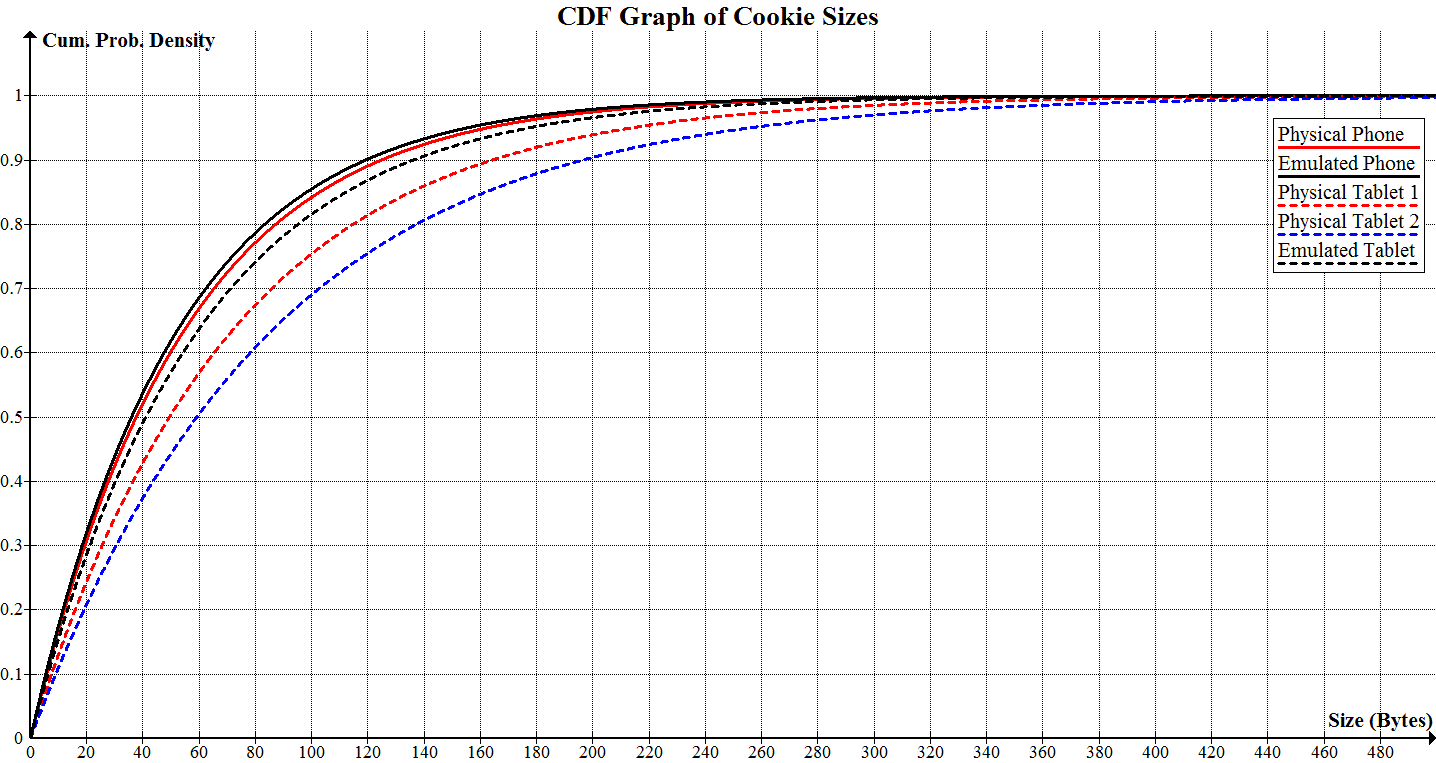
\includegraphics[scale=0.30]{diagrams/cookies_cdf.png}
\caption{Cookie size distribution with Top 500 dataset}
\label{fig:cookie_cdf}
\end{figure*}

\begin{figure*}[ht] 
\centering 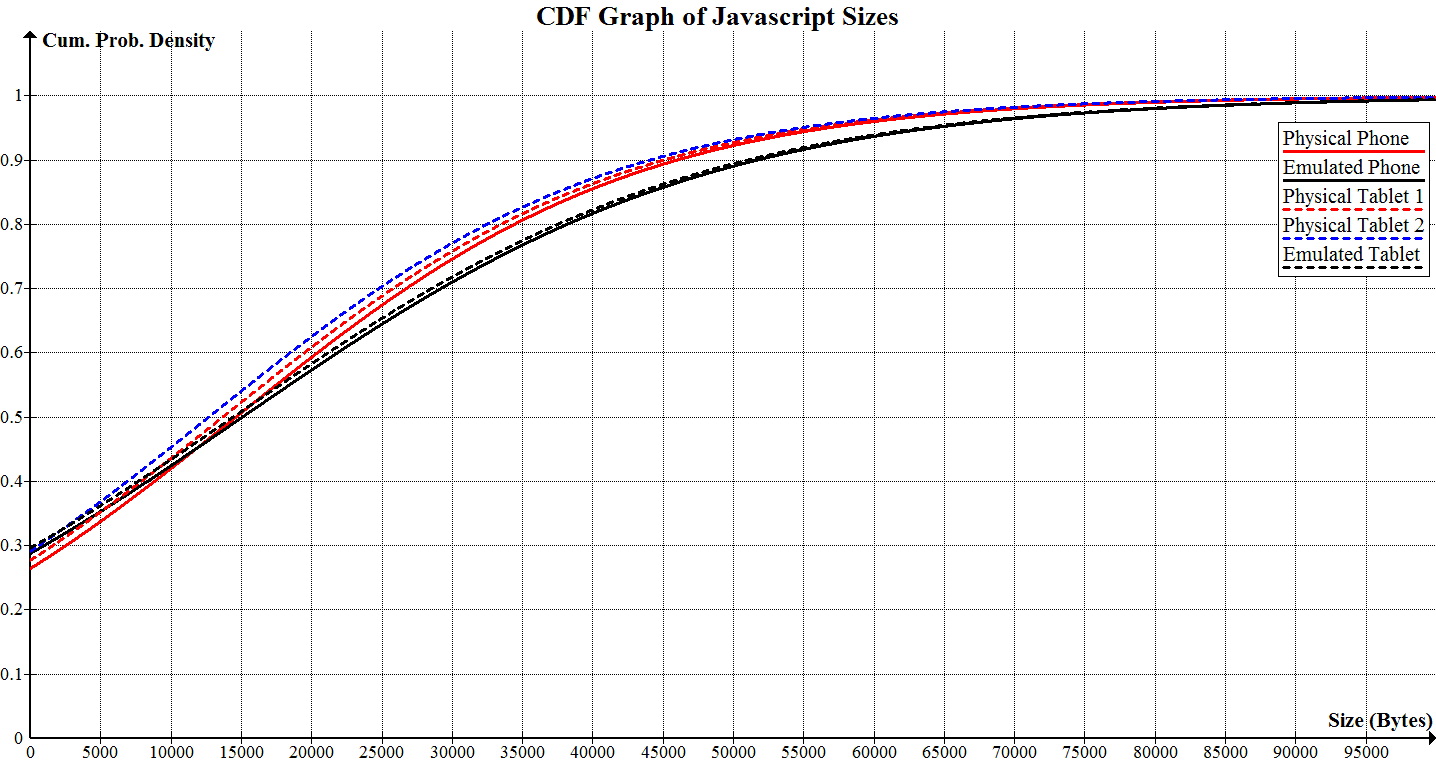
\includegraphics[scale=0.30]{diagrams/javascript_cdf.png}
\caption{JavaScript script size distribution with Top 500 dataset}
\label{fig:javascript_cdf}
\end{figure*}

There are three possible actions that can be taken when it comes to cookies: creation, modification and deletion. Tables \ref{tab:cookie_counts_100} and \ref{tab:cookie_counts_500} show the number of cookie events detected by our five mobile devices when crawling the Top 100 and Top 500 URL datasets respectively. It can be seen that the HTC Evo 4G and the Emulated Nexus S presented congruent numbers, while the three tablets appear to be remarkably dissimilar from one other.

Both datasets show the aforementioned trends, which are quantified in Table \ref{tab:cookie_deltas}, where the differences between the emulated and expected (physical) results are presented. In the case of tablets, the two physical devices were averaged and taken as the expected result. We found that the emulated phone only distanced itself from the real phone by 16.67\% or less in terms of the cookie action counts. The emulated tablet showed lower fidelity, being off by 55.73\% in some cases.

\begin{table}[htbp]
  \centering
  \caption{Cookie action counts with Top 100 dataset}
    \begin{tabular}{|c|c|c|c|}
    \hline
    \multicolumn{1}{|c|}{\multirow{2}[4]{*}{\textbf{Device}}} & \multicolumn{3}{|c|}{\textbf{Cookies - Top 100 Dataset}} \\ \cline{2-4}
    \multicolumn{1}{|c|}{} & \multicolumn{1}{|c|}{\textbf{Added}} & \multicolumn{1}{|c|}{\textbf{Changed}} & \multicolumn{1}{|c|}{\textbf{Deleted}} \\ \hline
    \multicolumn{1}{|l|}{\textbf{HTC Evo 4G}} & 936   & 1214  & 18 \\
    \multicolumn{1}{|l|}{\textbf{Emulated Nexus S}} & 929   & 1130  & 15 \\
    \multicolumn{1}{|l|}{\textbf{Asus Pad TF300T}} & 1093  & 1351  & 40 \\
    \multicolumn{1}{|l|}{\textbf{Samsung G. Tab 2}} & 1374  & 2494  & 107 \\
    \multicolumn{1}{|l|}{\textbf{Emulated Nexus 7}} & 1282  & 2029  & 97 \\ \hline
    \end{tabular}%
  \label{tab:cookie_counts_100}%
\end{table}%

\begin{table}[htbp]
  \centering
  \caption{Cookie action counts with Top 500 dataset}
    \begin{tabular}{|c|c|c|c|}
    \hline
    \multicolumn{1}{|c|}{\multirow{2}[4]{*}{\textbf{Device}}} & \multicolumn{3}{|c|}{\textbf{Cookies - Top 500 Dataset}} \\ \cline{2-4}
    \multicolumn{1}{|c|}{} & \multicolumn{1}{|c|}{\textbf{Added}} & \multicolumn{1}{|c|}{\textbf{Changed}} & \multicolumn{1}{|c|}{\textbf{Deleted}} \\ \hline
    \multicolumn{1}{|l|}{\textbf{HTC Evo 4G}} & 4387  & 4545  & 101 \\
    \multicolumn{1}{|l|}{\textbf{Emulated Nexus S}} & 4665  & 4946  & 100 \\
    \multicolumn{1}{|l|}{\textbf{Asus Pad TF300T}} & 5163  & 6190  & 205 \\
    \multicolumn{1}{|l|}{\textbf{Samsung G. Tab 2}} & 5630  & 7501  & 319 \\
    \multicolumn{1}{|l|}{\textbf{Emulated Nexus 7}} & 4501  & 5107  & 116 \\ \hline
    \end{tabular}%
  \label{tab:cookie_counts_500}%
\end{table}%

\begin{table}[htbp]
  \centering
  \caption{Emulated vs Physical deltas in terms of cookie action counts}
    \begin{tabular}{|c|c|c|c|c|}
    \hline
    \multicolumn{1}{|c|}{\multirow{2}[4]{*}{\textbf{Device}}} & \multicolumn{1}{|c|}{\multirow{2}[4]{*}{\textbf{Dataset}}} & \multicolumn{3}{|c|}{\textbf{Cookies}} \\ \cline{3-5}
    \multicolumn{1}{|c|}{} & \multicolumn{1}{|c|}{} & \multicolumn{1}{|c|}{\textbf{Added}} & \multicolumn{1}{|c|}{\textbf{Changed}} & \multicolumn{1}{|c|}{\textbf{Deleted}} \\ \hline
    \multicolumn{1}{|l|}{\multirow{2}[4]{*}{\textbf{Phone}}} & Top 100 & -0.75\% & -6.92\% & -16.67\% \\
    \multicolumn{1}{|l|}{} & Top 500 & 6.34\% & 8.82\% & -0.99\% \\
    \hline
    \multicolumn{1}{|l|}{\multirow{2}[4]{*}{\textbf{Tablet}}} & Top 100 & 3.93\% & 5.54\% & 31.97\% \\
    \multicolumn{1}{|l|}{} & Top 500 & -16.59\% & -25.40\% & -55.73\% \\ \hline
    \end{tabular}%
  \label{tab:cookie_deltas}%
\end{table}%


Besides having the same amount of cookie events as a physical device, it is important that an emulated device is exposed to cookies of similar nature. A basic way to categorize cookies is by their expiration time: some are evicted from the browser's memory after a finite amount of time, while others are meant to stay in the browser's memory permanently. Permanent cookies are set by Mozilla Firefox to expire after exactly $9.223372036854776*10^{18}$ milliseconds; temporary cookies have eviction times that are more manageable (e.g. 11 days). Table \ref{tab:cookie_longevity} gives the total count of permanent and temporary cookies found in crawls with the Top 500 dataset, as well as their relative proportions. Once more, the Emulated Nexus S mirrors the HTC Evo 4G's behavior fairly closely. To our surprise, the counts and nature of cookies reported by the Emulated Nexus 7 are almost the same as those of the Emulated Nexus S. As a result, the Emulated Nexus 7 is not a good replacement for either of the tablets under this criteria. Referring back to Table \ref{tab:cookie_counts_500}, we soon realized that the Emulated Nexus 7 has consistently been acting more like a phone than as a tablet when it comes to cookies.


\begin{table}[htbp]
  \centering
  \caption{Cookie longevity with Top 500 dataset}
    \begin{tabular}{|c|c|c|c|c|}
    \hline
    \multicolumn{1}{|c|}{\multirow{2}[4]{*}{\textbf{Device}}} & \multicolumn{4}{|c|}{\textbf{Cookies - Top 500 Dataset}} \\ \cline{2-5}
    \multicolumn{1}{|c|}{} & \textbf{Perm.} & \textbf{Temp.} & \textbf{\% Perm.} & \textbf{Total} \\ \hline
    \multicolumn{1}{|l|}{\textbf{HTC Evo 4G}} & 2805  & 6228  & 31.05\% & 9033 \\
    \multicolumn{1}{|l|}{\textbf{Emulated Nexus S}} & 3002  & 6709  & 30.91\% & 9711 \\
    \multicolumn{1}{|l|}{\textbf{Asus Pad TF300T}} & 3364  & 8194  & 29.11\% & 11558 \\
    \multicolumn{1}{|l|}{\textbf{Samsung G. Tab 2}} & 3779  & 9671  & 28.10\% & 13450 \\
    \multicolumn{1}{|l|}{\textbf{Emulated Nexus 7}} & 3014  & 6710  & 31.00\% & 9724 \\ \hline
    \end{tabular}%
  \label{tab:cookie_longevity}%
\end{table}%

Now that we analyzed cookies by their counts and their longevity, we can dig deeper and investigate their content. Cookie size is a good metric to use when looking at the overall trends, since it gives an idea of the cookie usage patterns employed by the content providers. While some websites can write a short ID to a user's cookie and maintain the user's profile on their back-end, other websites might want to use cookies as a side-channel and keep all relevant tracking information on the client's side, appending data to existing cookies.

Table \ref{tab:cookie_sizes} gives the average size of the cookies detected during the Top 500 crawls by the different mobile devices. Note that tablets reported a larger cookie size on average than phones. To improve our understanding of the cookie size distributions for the two platforms, we used 2R Soft\footnote{http://www.2rsoft.tk} to run a single-series analysis over the cookies associated with each crawl and used goodness-of-fit tests to select the best cumulative density function (CDF) fit. An exponential distribution gave the best Anderson-Darling statistic in all cases, with the parameters given in Table \ref{tab:cookie_sizes}. We plotted the five CDFs and obtained Figure \ref{fig:cookie_cdf}. Tablet crawls are represented with dotted lines and phone crawls are shown as solid lines. From the CDF curves, it is clear that the Emulated Phone (Nexus S) serves as a convincing approximation to the Physical Phone (HTC Evo 4G). Meanwhile, the Emulated Tablet (Nexus 7) remains closer to the phone crawls than to the real tablet crawls. Also, it should be noted that the two physical tablets (Asus TF300T and Samsung Galaxy Tab 2) show cookie sizes that tend to be larger than the ones registered in phones.

\begin{table}[htbp]
  \centering
  \caption{Cookie size distribution with Top 500 dataset}
    \begin{tabular}{|c|c|c|}
    \hline
    \multicolumn{1}{|c|}{\multirow{2}[4]{*}{\textbf{Device}}} & \multicolumn{2}{|c|}{\textbf{Cookies - Top 500 Dataset}} \\ \cline{2-3}
    \multicolumn{1}{|c|}{} & \textbf{Avg Size (B)} & \textbf{Best CDF Fit} \\ \hline
    \multicolumn{1}{|l|}{\textbf{HTC Evo 4G}} & 54.29 & Exp., $\lambda$=0.01842 \\
    \multicolumn{1}{|l|}{\textbf{Emulated Nexus S}} & 51.86 & Exp., $\lambda$=0.01928 \\
    \multicolumn{1}{|l|}{\textbf{Asus Pad TF300T}} & 71.37 & Exp., $\lambda$=0.01401 \\
    \multicolumn{1}{|l|}{\textbf{Samsung G. Tab 2}} & 85.37 & Exp., $\lambda$=0.01171 \\
    \multicolumn{1}{|l|}{\textbf{Emulated Nexus 7}} & 59.20 & Exp., $\lambda$=0.01689 \\ \hline
    \end{tabular}%
  \label{tab:cookie_sizes}%
\end{table}%

\subsubsection{HTTP Interactions}

We are interested in comparing the content served to the various mobile devices to determine if websites are effectively fooled by the device emulator. This comes down to the HTTP Responses reported by FourthPartyMobile, which most of the time contain a \emph{Content-Type} header indicating the MIME type of the response's payload. From the crawl databases, we found that a around half of the HTTP responses carried images in all of their formats (e.g. jpg, png, gif) and the other half was mostly comprised of text. We separate JavaScript from the other types of text-based content (e.g. html and plaintext) because, as mentioned before, it is an integral part of web tracking and browser fingerprinting. While we thought that Flash cookies would be of common use based on previous research \cite{FLASH_COOKIES}, none of our crawls conducted on mobile devices with the Top 500 dataset contained more than 24 flash-related HTTP responses. This may be due to the fact that mobile browsers disable plug-in content by default and download such content on-demand when the user clicks on it.

Tables \ref{tab:http_100} and \ref{tab:http_500} show the counts of the various content types obtained with the Top 100 and Top 500 datasets respectively. Images are clearly the predominant type of media associated with HTTP responses in all of the crawls. At first glance, the counts reported by the Emulated Nexus S are not very distant from those of the physical phone. The same can be said about the emulated tablet (Nexus 7) with respect to the counts of its physical counterparts (Asus Pad TF300T and Samsung Galaxy Tab 2), but only when dealing with the Top 100 dataset. The emulated tablet was less satisfactory in replicating what was seen in the physical tablets with the Top 500 dataset.

Table \ref{tab:http_diffs} summarizes the difference between the emulated and expected (physical) results. In the case of tablets, the two physical devices were averaged and taken as the expected result. Similar to what was seen with cookies, the emulated phone does not deviate considerably from our reference physical phone, with deltas of less than 8.33\% in all counts. While the behavior of the emulated tablet was unexpectedly close to what we desired with the Top 100 dataset, the larger dataset brought about deltas of around 20\% on all counts, which might be unacceptable. This would explain why, as discussed in the previous subsection, the emulated tablet did not behave the same way as the physical tablets in terms of cookie activity. After all, it appears that the emulated tablet did not receive the same web content that the physical tablets received.

\begin{table}[htbp]
  \centering
  \caption{HTTP Responses by content type, Top 100 dataset}
    \begin{tabular}{|c|c|c|c|c|c|}
    \hline
    \multicolumn{1}{|c|}{\multirow{2}[4]{*}{\textbf{Device}}} & \multicolumn{4}{|c|}{\textbf{HTTP Responses - Top 100}} \\ \cline{2-5}
    \multicolumn{1}{|c|}{} & \textbf{total} & \textbf{image} & \textbf{JS} & \textbf{other} \\ \hline
    \multicolumn{1}{|l|}{\textbf{HTC Evo 4G}} & 3710  & 2269  & 721   & 720 \\
    \multicolumn{1}{|l|}{\textbf{Emulated Nexus S}} & 3546  & 2208  & 678   & 660 \\
    \multicolumn{1}{|l|}{\textbf{Asus Pad TF300T}} & 4440  & 2708  & 914   & 818 \\
    \multicolumn{1}{|l|}{\textbf{Samsung G. Tab 2}} & 5460  & 3069  & 1294  & 1097 \\
    \multicolumn{1}{|l|}{\textbf{Emulated Nexus 7}} & 4743  & 2848  & 1007  & 888 \\ \hline
    \end{tabular}%
  \label{tab:http_100}%
\end{table}%

\begin{table}[htbp]
  \centering
  \caption{HTTP Responses by content type, Top 500 dataset}
    \begin{tabular}{|c|c|c|c|c|c|}
    \hline
    \multicolumn{1}{|c|}{\multirow{2}[4]{*}{\textbf{Device}}} & \multicolumn{4}{|c|}{\textbf{HTTP Responses - Top 500}} \\ \cline{2-5}
    \multicolumn{1}{|c|}{} & \textbf{total} & \textbf{image} & \textbf{JS} & \textbf{other} \\ \hline
    \multicolumn{1}{|l|}{\textbf{HTC Evo 4G}} & 17848 & 10932 & 3616  & 3300 \\
    \multicolumn{1}{|l|}{\textbf{Emulated Nexus S}} & 18376 & 11052 & 3870  & 3454 \\
    \multicolumn{1}{|l|}{\textbf{Asus Pad TF300T}} & 24283 & 15045 & 5131  & 4107 \\
    \multicolumn{1}{|l|}{\textbf{Samsung G. Tab 2}} & 27544 & 16664 & 6132  & 4748 \\
    \multicolumn{1}{|l|}{\textbf{Emulated Nexus 7}} & 20441 & 12735 & 4298  & 3408 \\
 \hline
    \end{tabular}%
  \label{tab:http_500}%
\end{table}%

\begin{table}[htbp]
  \centering
  \caption{Emulated vs Physical deltas in terms of HTTP response content types}
    \begin{tabular}{|c|c|c|c|c|c|}
    \hline
    \multicolumn{1}{|c|}{\multirow{2}[4]{*}{\textbf{Device}}} & \multicolumn{1}{|c|}{\multirow{2}[4]{*}{\textbf{Dataset}}} & \multicolumn{4}{|c|}{\textbf{HTTP Responses}} \\ \cline{3-6}
    \multicolumn{1}{|c|}{} & \multicolumn{1}{|c|}{} & \multicolumn{1}{|c|}{\textbf{total}} & \multicolumn{1}{|c|}{\textbf{image}} & \multicolumn{1}{|c|}{\textbf{JS}} & \multicolumn{1}{|c|}{\textbf{other}} \\ \hline
    \multicolumn{1}{|l|}{\multirow{2}[4]{*}{\textbf{Phone}}} & Top 100 & -4.42\% & -2.69\% & -5.96\% & -8.33\% \\
    \multicolumn{1}{|l|}{} & Top 500 & 2.96\% & 1.10\% & 7.02\% & 4.67\% \\ \hline
    \multicolumn{1}{|l|}{\multirow{2}[4]{*}{\textbf{Tablet}}} & Top 100 & -4.18\% & -1.40\% & -8.79\% & -7.26\% \\
    \multicolumn{1}{|l|}{} & Top 500 & -21.12\% & -19.68\% & -23.68\% & -23.03\% \\ \hline
    \end{tabular}%
  \label{tab:http_diffs}%
\end{table}%

\subsubsection{JavaScript Interactions}

A high-level picture of the JavaScript code that was executed in the mobile browsers can be drawn based on the size distribution of the scripts transmitted by the content providers. Larger scripts are likely to contain more lines of code, so they are expected to execute more powerful (or intrusive) procedures on the client-side.

Table \ref{tab:javascript_sizes} gives the average size in Bytes of the JavaScript files executed on each device during the Top 500 crawl. All averages have the same order of magnitude, so a more in-depth approach is in order.  Similar to what was done with the cookie sizes, we performed a best-fit analysis with the help of 2R Soft\footnote{http://www.2rsoft.tk} and selected the most appropriate cumulative density function (CDF). Judging by the Anderson-Darling statistic, all crawls are best represented by a logistic distribution with parameters given in Table \ref{tab:javascript_sizes}. The end results are plotted in Figure \ref{fig:javascript_cdf}. Interestingly, the two emulated devices have JavaScript size CDF curves that are closer to each other than to that of any of the physical devices. In addition, all three physical devices have practically the same JavaScript size CDF curve. Nonetheless, the distance between the curves associated with emulated devices and the curves associated with their physical counterparts is relatively small in comparison with what was seen in the cookie size CDFs (Figure \ref{fig:cookie_cdf}) when dealing with tablets.

\begin{table}[htbp]
  \centering
  \caption{JavaScript script size distribution, Top 500 dataset}
    \begin{tabular}{|c|c|p{2.3cm}|}
    \hline
    \multicolumn{1}{|c|}{\multirow{2}[4]{*}{\textbf{Device}}} & \multicolumn{2}{|c|}{\textbf{JavaScript - Top 500}} \\ \cline{2-3}
    \multicolumn{1}{|c|}{} & \textbf{Avg Size (B)} & \textbf{Best CDF Fit} \\ \hline
    \multicolumn{1}{|l|}{\textbf{HTC Evo 4G}} & 14,647.11 & \parbox{4cm}{Logistic,\\$\alpha$=14,647.11,\\$\lambda$=0.00007\\} \\ 
    \multicolumn{1}{|l|}{\textbf{Emulated Nexus S}} & 15,107.96 & \parbox{4cm}{Logistic,\\ $\alpha$=15,107.96,\\$\lambda$=0.00006\\} \\
    \multicolumn{1}{|l|}{\textbf{Asus Pad TF300T}} & 13,708.73 & \parbox{4cm}{Logistic,\\ $\alpha$=13,708.73,\\$\lambda$=0.00007\\} \\
    \multicolumn{1}{|l|}{\textbf{Samsung G. Tab 2}} & 12,711.00 & \parbox{4cm}{Logistic,\\ $\alpha$=12,711.00,\\$\lambda$=0.00007\\} \\
    \multicolumn{1}{|l|}{\textbf{Emulated Nexus 7}} & 14,445.22 & \parbox{4cm}{Logistic,\\ $\alpha$=14,445.22,\\$\lambda$=0.00006\\} \\ \hline
    \end{tabular}%
  \label{tab:javascript_sizes}%
\end{table}%

\subsubsection{Our Findings}
We believe that we have provided enough evidence to prove that an emulated phone (i.e. Emulated Nexus S) can impersonate a physical phone (i.e. HTC Evo 4G) with a great degree of accuracy. On the other hand, the Emulated Nexus 7 tablet consistently falls short when compared to what is expected from a physical tablet and most metrics seem to indicate that it is closer to mimicking an emulated phone than any of the physical devices.

\subsection{Privacy Policy Case Study}
After running our web crawls, we designed a case study in which we look at the privacy policies and related data collected from our crawls of three categories of websites that we found were amongst the most popular sites today: social networks, news sites, and e-commerce sites. While pornography sites are also amongst the most popular sites online, we do not include this fourth category in our case study for reasons of decency. 

Based on the list of the Alexa Top 100 US visited websites, we chose three websites amongst the top 25 most visited sites, one representing each of our three categories. Our case study examines the privacy policies of LinkedIn\footnote{http://www.linkedin.com} (social network), CNN\footnote{http://www.cnn.com} (news) and Amazon\footnote{http://www.amazon.com} (e-commerce).

The case study has four stages, each stage looking at the privacy policies in more detail:
\begin{enumerate}
\item Compare the contents of the privacy policies displayed when visiting each of the sites on our three platforms (desktop, tablet, and smartphone).
\item Compare the length of the privacy policies of each website.
\item Examine the topics covered, i.e., the sections included in the policies.
\item Inspect some of the language used in select sections of the policies.
\end{enumerate}

The question we wanted to answer in our case study was \emph{Do privacy policies vary between normal web and mobile web?} Thus, the first stage of the case study, seeks to answer this question via a very simple method. We visited the three websites on our three platforms and downloaded the presented privacy policies for each site on each platform. This gave us three privacy policies each for LinkedIn, CNN, and Amazon. 

The easiest and quickest way to determine if the contents of the policies differ for a single website was to run the \texttt{diff} command between the policies collected for each pair of platforms\footnote{The policies were all saved as text documents, and stripped of tabs and empty lines via a python script.}: desktop - smartphone, desktop - tablet, and tablet - smartphone. Taking the more pessimistic standpoint, we were expecting to find that a single website's policies would differ more between the three platforms. But what we discovered in reality is that in the cases of LinkedIn and CNN, the privacy policies for all three platforms are exactly identical. \textbf{keep this}We consider this to be a positive finding as this proves that the websites make an effort to maintain consistency across the devices.\textbf{??} In the case of Amazon, the privacy policies presented when visiting the website through a desktop and a tablet are exactly identical. However, the smartphone version of the policy is much shorter and refers the reader to the full (desktop) version of their privacy notice. We would like to note that the fact that the privacy policies were basically all identical for each of the three websites in our case study greatly facilitated our further analysis of the privacy policies. The remaining examinations discussed in this section were done using the desktop version of the policies.

Our next point of study was the length of each of the privacy policies as this is an indicator of the amount of detail the websites offer their visitors. Running the \texttt{wc -w} command on each website's policy. The the resulting word counts are summarized in Table \ref{tab:wc}.

\begin{table}[htbp]
  \centering
  \caption{Word counts of the privacy policies of our three studied websites.}
    \begin{tabular}{|c|c|}
    \hline
    \textbf{Website} & \textbf{Word Count} \\    
     \hline
     LinkedIn & 6324 \\
     CNN & 2734 \\
     Amazon & 2691 \\
     \hline
    \end{tabular}%
  \label{tab:wc}%
\end{table}%

We were not surprised to see that the social network has the longest privacy policy, as these types of websites are in a constant race to see who can protect their users' privacy better. Thus, longer and more detailed is better for social networks. However, we were also expecting the e-commerce site to have a longer privacy policy, given that users purchase items through these sites by inputting sensitive data such as credit card numbers and home addresses. Thus, we were expecting to see that the website would supply the user with more detailed information about their privacy practices to reassure them that especially their sensitive data will be dealt with appropriately. What we were not expecting was to find that Amazon would have the shortest policy of our three studied websites.

Once we had examined the privacy policies in terms of their length, we began to analyze them more carefully looking at the topics that they all cover, which are dedicated their own section in most cases. Figure \ref{fig:at-a-glance} shows a comparison of LinkedIn, CNN, and Amazon in terms of the sections these sites include in their privacy policies at a glance. For a full list of the sections, please refer to \cite{amazon,linkedin,cnn}.

\begin{figure} 
\centering
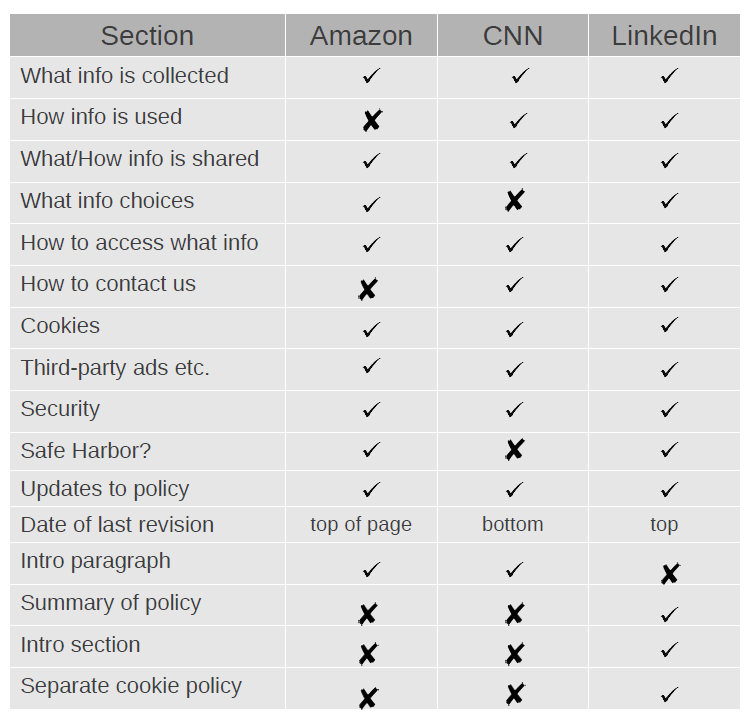
\includegraphics[width=0.5\textwidth]{at-a-glance}
\caption{The sections covered in the policies of all three studied sites at a glance. Check-marks denote the existence of a section, X-marks denote the absence of a section.}
\label{fig:at-a-glance}
\end{figure}

As can be seen in Figure \ref{fig:at-a-glance}, there are only eight topics which all three privacy policies in our case study cover, including the presence of the last revision date at some position on the web page. It is also important to note that the sections included in CNN's and Amazon's privacy policies correspond to one of the rows in Figure \ref{fig:at-a-glance}, while several of the topics marked as covered in this figure in the LinkedIn policy are in fact subsections of more general sections of their privacy policy. For instance, Section 2 in this privacy policy covers ``How LinkedIn uses your information.", where information sharing is discussed in Section 2.E and third-party content providers are explained in Section 2.K, while cookies are discussed in Section 1.G \cite{linkedin}.

LinkedIn's privacy policy includes a few other features that the other two policies do not have. CNN and Amazon both have short introductory paragraphs in which they state the purpose and mission to protect users' privacy at the beginning of the policy. For instance, CNN's introductory paragraph states the following: 
\begin{quotation}``Thank you for visiting CNN.com, a site presented to you by Turner Broadcasting System, Inc. ("Turner"). Your privacy is important to us. As such, we provide this privacy statement explaining our online information practices and the choices you can make about the way your information is collected and used at this general audience Turner site, and among Turner's network of affiliated websites ("Turner Network"), which includes any sites or services owned, operated or offered by or on behalf of Turner or its affiliates." \cite{cnn}\end{quotation}


A brief statement like this serves the purpose to appease readers who may not want to read through the entire privacy policy, and who are satisfied by knowing that the website even presents such a document.

LinkedIn, on the other hand, include a short ``Privacy Policy Highlights" section at the top of the web page, which summarizes the full privacy policy. This summary is great for users who do not want to go through the entire p\pp but still want to get a general idea of the information contained in the \pp. Furthermore, the logo of TRUSTe\footnote{TRUSTe is a global data privacy management solutions provider, part of whose mission is to ensure that digital businesses comply with international privacy requirements \cite{truste}.} EU Safe Harbor and a link to the TRUSTe ``Click to Verify" page is displayed at the top of the \pp web page. This TRUSTe website seal verifies that LinkedIn's privacy practices comply with TRUSTe's standards \cite{truste}.

Additionally, there are a few sections which we consider to be specific to a particular website category. In the case of LinkedIn, this is Section 4 ``Your obligations", which outlines the guidelines users on the social network need to abide to in order to maintain a valid account \cite{linkedin}. CNN includes three extra sections that are notably related to the fact that this is a news site belonging to a larger broadcasting corporation, namely ``Ad Choices", ``Turner's Participation in the Industry Self Regulatory Program for Interest Based Ads; Additional Choice Options", and ``International Transfer" \cite{cnn}. These sections mainly discuss additional practices of the broader Turner Network. Similarly to LinkedIn, Amazon's privacy policy also includes a ``Conditions of Use, Notices, and Revisions" section, in which the website not only advises users to check regularly for changes to the policy but also refers users to Amazon's ``Conditions of Use" web page and other informative pages \cite{amazon}.

At this stage of the case study, it became clear to us that we needed more than just to examine the sections covered in the \pps. Thus, the fourth phase of was to investigate the language used in select sections of the \pps. We decided to focus on the ``Cookies", and the ``Security" sections of the policies of the three websites.

One intriguing feature to examine in the ``Cookies" sections is the definition of \textit{cookie} that the websites present in their \pps. Table \ref{tab:cookie-defs} summarizes the definitions found in \cite{amazon,linkedin,cnn}.

\begin{table}[htbp]
  \centering
  \caption{The definitions of \textit{cookie} in the \pps of our three studied websites.}
    \begin{tabular}{|c|p{6.5cm}|}
    \hline
    \textbf{Website} & \textbf{Definition} \\    
     \hline
     LinkedIn &  A cookie is a tiny data file that resides on your computer, mobile phone, or other device, and allows us to recognize you as a User when you return to the LinkedIn website using the same computer and web browser. \\
     \hline
     CNN & Cookies are text files placed in your computer's browser to store your preferences. Cookies do not contain personally identifiable information; however, once you choose to furnish a site with personally identifiable information, this information may be linked to the data stored in the cookie. \\
\hline
     Amazon & Cookies are unique identifiers that we transfer to your device to enable our systems to recognize your device and to provide features such as 1-Click purchasing, Recommended for You, personalized advertisements on other Web sites (e.g., Amazon Associates with content served by Amazon.com and Web sites using Checkout by Amazon payment service), and storage of items in your Shopping Cart between visits.  \\
     \hline
    \end{tabular}%
  \label{tab:cookie-defs}%
\end{table}%

One can see that the definitions of \textit{cookie} are driven by each website's primary usage of cookies. Both LinkedIn and Amazon state that the main purpose of cookies is to remember a user that has once visited the website before. One the other hand, CNN simply seems to use cookies for personalization purposes, so that is the definition they offer. It is also interesting to see that the cookie itself is described in three different ways: as a ``tiny data file", as a ``text file", and also as a ``unique identifier". This, for instance, is an indication that uniformity across all websites would be useful to avoid any kind of confusion among laypeople. 

The other section we investigated in more detail was the ``Security" section of all the \pps. Amazon and LinkedIn mention SSL encryption directly \cite{amazon,linkedin}, while CNN is very vague and simply states: ``We have put in place appropriate physical, electronic, and managerial procedures to safeguard and help prevent unauthorized access, to maintain data security, and to use correctly the information we collect online" \cite{cnn}. It is unclear whether or not CNN even uses any kind of encryption at all, although due to the nature of the website, it is possible that this site may not require the encryption of any information. We did not study the extent to which this may be true. However, by simply clicking on the ``Log in" link, it does not seem as if this page is transmitted via HTTPS. Nonetheless, it makes sense for the other two websites to use SSL encryption since their website categories by nature require users to input and submit much more sensitive data, such as credit card numbers, and other personal information. The other issue with CNN's language is the fact that it is overly non-technical, which may imply that the authors of the \pp may simply not have technical knowledge. This is another sign that it may be helpful for policymakers to receive some technical education, which would make \pps more uniform and informative.

In the end, we can conclude based on the first three stages of our case study that LinkedIn's meticulously written privacy policy is the most useful for various kinds of users. Their privacy summary is an incredibly helpful tool, especially for those users who want to be informed about what their social network is doing with respect to their data and privacy, but do not or cannot take the time to read through the entire document. In addition, the fact that LinkedIn also includes a separate Cookie Policy shows that they put the time into creating documents that would fully inform their users. Another intriguing case study would be to compare LinkedIn's \pp with that of other social networks to see if our conclusion about \pps of social networks holds. 

The lessons learned in the last stage of our case study are two-fold: (1) \pps are clearly tailored to each of the studied website's main purposes and goals, and (2) more consistency is required in the \pps across website categories to avoid confusion. While we agree that \pps need to reflect a website's purpose and goals, we also argue that the extent of the discrepancies, particularly in the sections studied, may call for more uniformity across \pps, and indicates the potential need for more communication between policymakers and the technology community. Nevertheless, we these lessons are drawn in limited premises due to time contraints, and we suggest that stage four of our case study be carried out in more deatil, potentially as its own case study in the future.

We hope that our analysis of the \pps of the three websites chosen for our case study will serve as a starting point for further conversation on the creation of \pps and privacy standards.

\section{Conclusions and Future Work}

\nocite{*}
\bibliographystyle{abbrv}
\bibliography{sigproc}
\end{document}
